\chapter{Optimization Capabilities}\label{opt}

Optimization algorithms work to minimize (or maximize) an objective
function, typically calculated by the user simulation code, subject to
constraints on design variables and responses. Available approaches
in Dakota include well-tested, proven gradient-based, derivative-free
local, and global methods, for use in science and engineering design
applications. Dakota also offers more advanced algorithm, e.g., to
manage multi-objective optimization or perform surrogate-based minimization.
This chapter summarizes optimization problem formulation, standard
algorithms available in Dakota (mostly through included third-party
libraries), some advanced capabilities, and offers usage guidelines.

\section{Optimization Formulations}\label{opt:formulations}

This section provides a basic introduction to the mathematical
formulation of optimization, nonlinear least squares, sensitivity
analysis, design of experiments, and uncertainty quantification
problems. The primary goal of this section is to introduce terms
relating to these topics, and is not intended to be a description of
theory or numerical algorithms. For further details,
consult~\cite{Aro89},~\cite{Gil81},~\cite{Haf92},~\cite{Noc99}, and
~\cite{Van84}.

A general optimization problem is formulated as follows:

\begin{eqnarray}
  \hbox{minimize:} & & f(\mathbf{x})\nonumber\\
  & & \mathbf{x} \in \Re^{n}\nonumber\\
  \hbox{subject to:} & &
  \mathbf{g}_{L} \leq \mathbf{g(x)} \leq \mathbf{g}_U\nonumber\\
  & & \mathbf{h(x)}=\mathbf{h}_{t}\label{opt:equation01}\\
  & & \mathbf{a}_{L} \leq \mathbf{A}_i\mathbf{x} \leq
  \mathbf{a}_U\nonumber\\
  & & \mathbf{A}_{e}\mathbf{x}=\mathbf{a}_{t}\nonumber\\
  & & \mathbf{x}_{L} \leq \mathbf{x} \leq \mathbf{x}_U\nonumber
\end{eqnarray}

where vector and matrix terms are marked in bold typeface. In this
formulation, $\mathbf{x}=[x_{1},x_{2},\ldots,x_{n}]$ is an
n-dimensional vector of real-valued \emph{design variables} or
\emph{design parameters}. The n-dimensional vectors, $\mathbf{x}_{L}$
and $\mathbf{x}_U$, are the lower and upper bounds, respectively, on
the design parameters. These bounds define the allowable values for
the elements of $\mathbf{x}$, and the set of all allowable values is
termed the \emph{design space} or the \emph{parameter space}. A
\emph{design point} or a \emph{sample point} is a particular set of 
values within the parameter space.

The optimization goal is to minimize the \emph{objective function},
$f(\mathbf{x})$, while satisfying the constraints. Constraints can be
categorized as either linear or nonlinear and as either inequality or
equality. The \emph{nonlinear inequality constraints},
$\mathbf{g(x)}$, are ``2-sided,'' in that they have both lower and
upper bounds, $\mathbf{g}_L$ and $\mathbf{g}_U$, respectively. The
\emph{nonlinear equality constraints}, $\mathbf{h(x)}$, have target
values specified by $\mathbf{h}_{t}$. The linear inequality
constraints create a linear system $\mathbf{A}_i\mathbf{x}$, where
$\mathbf{A}_i$ is the coefficient matrix for the linear system. These
constraints are also 2-sided as they have lower and upper bounds,
$\mathbf{a}_L$ and $\mathbf{a}_U$, respectively. The linear equality
constraints create a linear system $\mathbf{A}_e\mathbf{x}$, where
$\mathbf{A}_e$ is the coefficient matrix for the linear system and
$\mathbf{a}_{t}$ are the target values. The constraints partition the
parameter space into feasible and infeasible regions. A design point
is said to be \emph{feasible} if and only if it satisfies all of the
constraints. Correspondingly, a design point is said to be
\emph{infeasible} if it violates one or more of the constraints.

Many different methods exist to solve the optimization problem given
by Equation~\ref{opt:equation01}, all of which iterate on
$\mathbf{x}$ in some manner. That is, an initial value for each
parameter in $\mathbf{x}$ is chosen, the \emph{response quantities},
$f(\mathbf{x})$, $\mathbf{g(x)}$, $\mathbf{h(x)}$, are computed, often
by running a simulation, and some algorithm is applied to generate a
new $\mathbf{x}$ that will either reduce the objective function,
reduce the amount of infeasibility, or both. To facilitate a general
presentation of these methods, three criteria will be used in the
following discussion to differentiate them: optimization problem type,
search goal, and search method.

The {\bf optimization problem type} can be characterized both by
the types of constraints present in the problem and by the linearity
or nonlinearity of the objective and constraint functions. For
constraint categorization, a hierarchy of complexity exists for
optimization algorithms, ranging from simple bound constraints,
through linear constraints, to full nonlinear constraints. By the
nature of this increasing complexity, optimization problem
categorizations are inclusive of all constraint types up to a
particular level of complexity. That is, an \emph{unconstrained
  problem} has no constraints, a \emph{bound-constrained problem} has
only lower and upper bounds on the design parameters, a
\emph{linearly-constrained problem} has both linear and bound
constraints, and a \emph{nonlinearly-constrained problem} may contain
the full range of nonlinear, linear, and bound constraints. If all of
the linear and nonlinear constraints are equality constraints, then
this is referred to as an \emph{equality-constrained problem}, and if
all of the linear and nonlinear constraints are inequality
constraints, then this is referred to as an
\emph{inequality-constrained problem}. Further categorizations can be
made based on the linearity of the objective and constraint functions.
A problem where the objective function and all constraints are linear
is called a \emph{linear programming (LP) problem}. These types of
problems commonly arise in scheduling, logistics, and resource
allocation applications. Likewise, a problem where at least some of
the objective and constraint functions are nonlinear is called a
\emph{nonlinear programming (NLP) problem}. These NLP problems
predominate in engineering applications and are the primary focus of
Dakota.

The {\bf search goal} refers to the ultimate objective of the
optimization algorithm, i.e., either global or local optimization. In
\emph{global optimization}, the goal is to find the design point that
gives the lowest feasible objective function value over the entire
parameter space. In contrast, in \emph{local optimization}, the goal
is to find a design point that is lowest relative to a ``nearby''
region of the parameter space. In almost all cases, global
optimization will be more computationally expensive than local
optimization. Thus, the user must choose an optimization algorithm
with an appropriate search scope that best fits the problem goals and
the computational budget.

The {\bf search method} refers to the approach taken in the
optimization algorithm to locate a new design point that has a lower
objective function or is more feasible than the current design point.
The search method can be classified as either \emph{gradient-based} or
\emph{nongradient-based}. In a gradient-based algorithm, gradients of
the response functions are computed to find the direction of
improvement. Gradient-based optimization is the search method that
underlies many efficient local optimization methods. However, a
drawback to this approach is that gradients can be computationally
expensive, inaccurate, or even nonexistent. In such situations,
nongradient-based search methods may be useful. There are numerous
approaches to nongradient-based optimization. Some of the more well
known of these include pattern search methods (nongradient-based local
techniques) and genetic algorithms (nongradient-based global
techniques). 

Because of the computational cost of running simulation
models, surrogate-based optimization (SBO) methods are often used to
reduce the number of actual simulation runs. In SBO, a surrogate or
approximate model is constructed based on a limited number of
simulation runs. The optimization is then performed on the surrogate
model. Dakota has an extensive framework for managing a variety of
local, multipoint, global, and hierarchical surrogates for use in
optimization. Finally, sometimes there are multiple objectives that 
one may want to optimize simultaneously instead of a single scalar 
objective.  In this case, one may employ multi-objective methods 
that are described in Section~\ref{opt:additional:multiobjective}.

This overview of optimization approaches underscores that no single
optimization method or algorithm works best for all types of
optimization problems. Section~\ref{opt:usage} offers guidelines for
choosing a Dakota optimization algorithm best matched to your specific
optimization problem.

\section{Optimizing with Dakota}\label{opt:dakota}

Dakota's input commands permit the user to specify two-sided nonlinear
inequality constraints of the form $g_{L_{i}} \leq g_{i}(\mathbf{x})
\leq g_{U_{i}}$, as well as nonlinear equality constraints of the form
$h_{j}(\mathbf{x}) = h_{t_{j}}$ (see also
Section~\ref{opt:formulations}). Some optimizers
(e.g., NPSOL, OPT++, JEGA) can handle these constraint forms directly,
whereas other optimizers (e.g., HOPSPACK, DOT, CONMIN) require Dakota
to perform an internal conversion of all constraints to one-sided
inequality constraints of the form $g_{i}(\mathbf{x}) \leq 0$. In the
latter case, the two-sided inequality constraints are treated as
$g_{i}(\mathbf{x}) - g_{U_{i}} \leq 0$ and $g_{L_{i}} -
g_{i}(\mathbf{x}) \leq 0$ and the equality constraints are treated as
$h_{j}(\mathbf{x}) - h_{t_{j}} \leq 0$ and $h_{t_{j}} -
h_{j}(\mathbf{x}) \leq 0$. The situation is similar for linear
constraints: HOPSPACK, NPSOL, OPT++, and JEGA support them directly,
whereas DOT and CONMIN do not. For linear inequalities of the form
$a_{L_{i}} \leq \mathbf{a}_{i}^{T}\mathbf{x} \leq a_{U_{i}}$ and
linear equalities of the form $\mathbf{a}_{i}^{T}\mathbf{x} =
a_{t_{j}}$, the nonlinear constraint arrays in DOT and CONMIN are
further augmented to include $\mathbf{a}_{i}^{T}\mathbf{x} - a_{U_{i}}
\leq 0$ and $a_{L_{i}} - \mathbf{a}_{i}^{T}\mathbf{x} \leq 0$ in the
inequality case and $\mathbf{a}_{i}^{T}\mathbf{x} - a_{t_{j}} \leq 0$
and $a_{t_{j}} - \mathbf{a}_{i}^{T}\mathbf{x} \leq 0$ in the equality
case. Awareness of these constraint augmentation procedures can be
important for understanding the diagnostic data returned from the DOT
and CONMIN algorithms. Other optimizers fall somewhere in between.
NLPQL supports nonlinear equality constraints $h_{j}(\mathbf{x}) = 0$
and nonlinear one-sided inequalities $g_{i}(\mathbf{x}) \geq 0$, but
does not natively support linear constraints. Constraint mappings are
used with NLPQL for both linear and nonlinear cases. Most SCOLIB
methods now support two-sided nonlinear inequality constraints and
nonlinear constraints with targets, but do not natively support linear
constraints. Constraint augmentation is not currently used with
SCOLIB since linear constraints will soon be supported natively.

When gradient and Hessian information is used in the optimization,
derivative components are most commonly computed with respect to the
active continuous variables, which in this case are the
\emph{continuous design variables}. This differs from parameter study
methods (for which all continuous variables are active) and from
nondeterministic analysis methods (for which the uncertain variables
are active). Refer to Section~\ref{responses:active} for additional
information on derivative components and active continuous variables.

\section{Optimization Software Packages}\label{opt:software}

This section summarizes the optimization packages available in Dakota,
which offers gradient-based local as well as derivative-free
approaches. For guidance selecting from the available packages, see
Section~\ref{opt:usage}. {\em Note that the DOT, NLPQL, and NPSOL
  packages are commercially licensed and not included in the open
  source version of Dakota. However a user of open source Dakota may
  obtain a software license and source code for them separately and
  then compile them into Dakota.}  The remainder of the packages
discussed here have licenses compatible with Dakota's and are
distributed in all Dakota releases.

\subsection{HOPSPACK}\label{opt:software:hopspack}

\textbf{HOPSPACK}: is a library that enables the implementation of
hybrid optimization algorithms~\cite{Plantenga2009}. Currently the
only method exposed is an asynchronous implementation of generating
set search known as asynchronous parallel pattern search
(APPS)~\cite{GrKo06}, available as method
\texttt{asynch\_pattern\_search}. APPS can handle unconstrained
problems as well as those with bound constraints, linear
constraints~\cite{GrKoLe08}, and general nonlinear
constraints~\cite{GrKo07}. APPS is best suited for simulation-based
problems with less than 100 variables. It has significant advantages
over gradient-based methods when the function is noisy and/or
discontinuous. APPS and HOPSPACK leverage the cddlib
software~\cite{Fu05} to handle degeneracy in linear constraints. {\em
  APPS was previously integrated with Dakota via the APPSPACK
  software, but is now integrated through it's HOPSPACK successor.}
License: LGPL; web page: \url{https://software.sandia.gov/trac/hopspack}.

An example specification for APPS with nonlinear constraints is:
\begin{small}
\begin{verbatim}
    method,
          asynch_pattern_search
             initial_delta = .5
             contraction_factor = 0.25
             threshold_delta = 1.e-4
             merit_function merit_max
             smoothing_factor = 10.0
\end{verbatim}
\end{small} % Could instead extract dakota_apps.in:5 to get most of this.

See the Dakota Reference Manual~\cite{RefMan} for additional detail on
the APPS commands and sample input specifications in {\tt
Dakota/test/dakota\_apps.in}.

\subsection{SCOLIB}\label{opt:software:coliny}

\textbf{SCOLIB}: The SCOLIB (formerly COLINY) library~\cite{Har06}
includes methods for derivative-free local and global optimization
which utilize the Common Optimization Library INterface (COLIN) of
ACRO (A Common Repository for Optimizers). License: BSD; web page:
\url{http://software.sandia.gov/trac/acro}.

SCOLIB optimizers currently available in Dakota include:
\begin{itemize}

\item {\bf Global Optimization Methods}
  \begin{itemize}
  \item Several evolutionary algorithms, including genetic algorithms
    (\texttt{coliny\_ea})
  \item DIRECT~\cite{Per93} (\texttt{coliny\_direct})
  \end{itemize}

\item {\bf Local Optimization Methods}
  \begin{itemize}
  \item Solis-Wets (\texttt{coliny\_solis\_wets})
  \item Pattern Search (\texttt{coliny\_pattern\_search})
  \end{itemize}

\item {\bf Interfaces to Third-Party Local Optimization Methods}
  \begin{itemize}
  \item COBYLA2 (\texttt{coliny\_cobyla})
  \end{itemize}

\end{itemize}
In addition, SCOLIB has capabilities for evolutionary pattern search
and Monte Carlo sampling, which are not available through Dakota.

For expensive optimization problems, SCOLIB's global optimizers are
best suited for identifying promising regions in the global design
space. In multimodal design spaces, the combination of global
identification (from SCOLIB) with efficient local convergence (from
CONMIN, DOT, NLPQL, NPSOL, or OPT++) can be highly effective. None of
the SCOLIB methods are gradient-based, which makes them appropriate
for problems for which gradient information is unavailable or is of
questionable accuracy due to numerical noise. The SCOLIB methods
support bound constraints and nonlinear constraints, but not linear
constraints. The nonlinear constraints in SCOLIB are currently
satisfied using penalty function formulations~\cite{Pon96}. Support
for methods which manage constraints internally is currently being
developed and will be incorporated into future versions of Dakota.
\emph{Note that one observed drawback to \texttt{coliny\_solis\_wets}
is that it does a poor job solving problems with nonlinear
constraints}. Refer to Table 17.1 for additional method
classification information.

An example specification for a simplex-based pattern search algorithm
from SCOLIB is:
\begin{small}
\begin{verbatim}
    method,
          coliny_pattern_search
            max_function_evaluations = 2000
            solution_accuracy = 1.0e-4
            initial_delta = 0.05
            threshold_delta = 1.0e-8
            pattern_basis simplex
            exploratory_moves adaptive_pattern
            contraction_factor = 0.75
\end{verbatim}
\end{small}

The Dakota Reference Manual~\cite{RefMan} contains additional information
on the SCOLIB options and settings and examples are shown in 
Section~\ref{opt:examples:ps} (pattern search) and
Section~\ref{opt:examples:ea} (evolutionary algorithm).

\subsection{Constrained Minimization (CONMIN)}\label{opt:software:conmin}

CONMIN~\cite{Van78} contains two methods for gradient-based nonlinear
optimization. For constrained optimization, the Method of Feasible
Directions (Dakota's \texttt{conmin\_mfd} method selection) is
available, while for unconstrained optimization, the Fletcher-Reeves
conjugate gradient method (Dakota's \texttt{conmin\_frcg} method
selection) is available. Both of these methods are most efficient at
finding a local minimum in the vicinity of the starting point. The
methods in CONMIN can be applied to global optimization problems, but
there is no guarantee that they will find the globally optimal design
point. License: Public Domain (NASA).

\emph{One observed drawback to CONMIN's Method of Feasible Directions
is that it does a poor job handling equality constraints}. This is the
case even if the equality constraint is formulated as two inequality
constraints. This problem is what motivates the modifications to MFD
that are present in DOT's MMFD algorithm. For problems with equality
constraints, it is better to use the OPT++ nonlinear interior point
methods, NPSOL, NLPQL, or one of DOT's constrained optimization
methods (see below).

An example specification for CONMIN's Method of Feasible Directions
algorithm is:
\begin{small}
\begin{verbatim}
    method,
          conmin_mfd
            convergence_tolerance = 1.0e-4
            max_iterations = 100
            output quiet
\end{verbatim}
\end{small}

Refer to the Dakota Reference Manual~\cite{RefMan} for more information on
the settings that can be used with CONMIN methods. An example using this method
is included in Section~\ref{additional:textbook:examples:gradient2}.

\subsection{Design Optimization Tools (DOT)}\label{opt:software:dot}

DOT has methods for gradient-based optimization for constrained and
unconstrained nonlinear optimization problems ~\cite{Van95}. For
unconstrained optimization, Dakota exposes the
Broyden-Fletcher-Goldfarb-Shanno (Dakota's \texttt{dot\_bfgs} method
selection) and Fletcher-Reeves conjugate gradient (Dakota's
\texttt{dot\_frcg} method selection) method. For constrained
optimization, we have the modified method of feasible directions
(Dakota's \texttt{dot\_mmfd} method selection), sequential linear
programming (Dakota's \texttt{dot\_slp} method selection), and
sequential quadratic programming (Dakota's \texttt{dot\_sqp} method
selection). License: commercial; website: Vanderplaats Research and
Development, \url{http://www.vrand.com}. {\em Sandia National
  Laboratories and Los Alamos National Laboratory have limited seats
  for DOT. Other users may obtain their own copy of DOT and compile it
  with the Dakota source code.}

All DOT methods are local gradient-based optimizers which are best
suited for efficient navigation to a local minimum in the vicinity of
the initial point. Global optima in nonconvex design spaces may be
missed. Other gradient based optimizers for constrained optimization
include the NPSOL, NLPQL, CONMIN, and OPT++ libraries.

Through the \texttt{optimization\_type} specification, DOT can be used
to solve either minimization or maximization problems. For all other
optimizer libraries, it is up to the user to reformulate a
maximization problem as a minimization problem by negating the
objective function (i.e., maximize $f(x)$ is equivalent to minimize
$-f(x)$). An example specification for DOT's BFGS quasi-Newton
algorithm is:
\begin{small}
\begin{verbatim}
    method,
          dot_bfgs
            optimization_type maximize
            convergence_tolerance = 1.0e-4
            max_iterations = 100
            output quiet
\end{verbatim}
\end{small}

\emph{We here provide a caution regarding \texttt{dot\_frcg}. In DOT
Version 4.20, we have noticed inconsistent behavior of this algorithm
across different versions of Linux. Our best assessment is that it is
due to different treatments of uninitialized variables. As we do not
know the intention of the code authors and maintaining DOT source code
is outside of the Dakota project scope, we have not made nor are we
recommending any code changes to address this. However, all users who
use \texttt{dot\_frcg} in DOT Version 4.20 should be aware that
results may not be reliable.}

See the Dakota
Reference Manual~\cite{RefMan} for additional detail on the DOT
commands. 

\subsection{dl\_solver --- Solvers via Shared Libraries}\label{opt:software:dlsolver}

On computer systems that permit use of shared libraries (most modern systems),
Dakota can avail itself of optimization solvers contained in shared libraries.
This is a first step toward allowing optional parts of Dakota, such as
proprietary solvers, to be accessed from shared libraries. For example,
the Dakota source distributions illustrate making
a sample shared-library interface to SNOPT~\cite{GilMS05},
whose use would be specified by
\begin{small}
\begin{verbatim}
    method,
          dl_solver = 'dl_snopt.dll'
\end{verbatim}
\end{small}
The quoted string contains the name of the shared library, optionally
followed by keyword assignments known to the library, such as
\begin{small}
\begin{verbatim}
    method,
          dl_solver = 'dl_snopt.dll outlev = 1'
\end{verbatim}
\end{small}
which would turn on some diagnostic printing in the SNOPT example.

\subsection{JEGA}\label{opt:software:jega}

% BMA: Text to consider integrating with below

% The MOGA package allows for the formulation of multiobjective
% optimization problems without the need to specify weights on the
% various objective function values. The MOGA method directly identifies
% non-dominated design points that lie on the Pareto front through
% tailoring of its genetic search operators. The advantage of the MOGA
% method versus conventional multiobjective optimization with weight
% factors, is that MOGA finds points along the entire Pareto front
% whereas the multiobjective optimization method produces only a single
% point on the Pareto front. The advantage of the MOGA method versus the
% Pareto-set optimization strategy is that MOGA is better able to find
% points on the Pareto front when the Pareto front is
% nonconvex. However, the use of a GA search method in MOGA causes the
% MOGA method to be much more computationally expensive than
% conventional multiobjective optimization using weight factors.

The JEGA (John Eddy's Genetic Algorithms) library contains two global
optimization methods. The first is a Multi-objective Genetic Algorithm
(MOGA) which performs Pareto optimization. The second is a
Single-objective Genetic Algorithm (SOGA, Dakota method \texttt{soga})
which performs optimization on a single objective function, using many
of the same software features as MOGA. The license for JEGA is LGPL.

The Dakota \texttt{moga} algorithm directly creates a population of
Pareto optimal solutions. Over time, the selection operators of a
genetic algorithm act to efficiently select non-dominated solutions
along the Pareto front. Because a GA involves a population of
solutions, many points along the Pareto front can be computed in a
single study. Thus, although GAs are computationally expensive when
compared to gradient-based methods, the advantage in the
multiobjective setting is that one can obtain an entire Pareto set at
the end of one genetic algorithm run, as compared with having to run
the ``weighted sum'' single objective problem multiple times with
different weights (Section~\ref{opt:additional:multiobjective}).

The Dakota Reference Manual~\cite{RefMan} contains additional
information on the JEGA options and settings.
Section~\ref{opt:additional} discusses additional multiobjective
optimization capabilities, and there are MOGA examples in
Chapters~\ref{tutorial} and~\ref{additional}.

%\subsection{MOOCHO Library}\label{opt:software:moocho}

%\textbf{MOOCHO (Multifunctional Object-Oriented arCHitecture for
%Optimization)}: formerly known as rSQP++, MOOCHO provides both
%general-purpose gradient-based algorithms for nested analysis and
%design (NAND) and large-scale gradient-based optimization algorithms
%for simultaneous analysis and design (SAND). This software is not yet
%distributed with Dakota.

%The MOOCHO (Multifunctional Object-Oriented arCHitecture for
%Optimization) library, formerly known as rSQP++, is a new addition to
%Dakota that is not yet publicly available. It provides both
%general-purpose sequential quadratic programming (SQP) algorithms for
%nested analysis and design (NAND) as well as reduced-space SQP
%algorithms for simultaneous analysis and design (SAND). Additional
%information on SAND is provided in Section~\ref{opt:additional:sand}.
%MOOCHO algorithm capabilities are available using the
%\texttt{reduced\_sqp} method selection.

\subsection{NCSU DIRECT}\label{opt:software:ncsu}

Dakota includes an NCSU implementation of the derivative-free global
optimization method called DIRECT (DIviding RECTangles algorithm),
detailed in~\cite{Gab01}. DIRECT is a derivative free global
optimization method that balances local search in promising regions of
the design space with global search in unexplored regions. DIRECT
adaptively subdivides the space of feasible design points to guarantee
that iterates are generated in the neighborhood of a global minimum in
finitely many iterations. In practice, DIRECT has proven an effective
heuristic for many applications, and for some problems, the NCSU
implementation has outperformed the SCOLIB version. License: MIT;
website: \url{http://www4.ncsu.edu/~ctk/matlab_darts.html}

NCSU DIRECT is specified with \texttt{ncsu\_direct}. One of the
controls is \texttt{volume\_boxsize\_limit}, which terminates the
optimization when the volume of the particular rectangle which contains
the minimum function value found thus far
is less than a certain percentage (given by the volume boxsize limit) of
the whole volume of the hyperrectangle defined by the variable bounds.
An example specification is given below:
\begin{small}
\begin{verbatim}
    method,
          ncsu_direct
          volume_boxsize_limit = 1.e-8
\end{verbatim}
\end{small}

The Dakota Reference Manual~\cite{RefMan} contains additional
information on the NCSU DIRECT options and settings.

\subsection{NLPQL}\label{opt:software:nlpql}

The NLPQL library for gradient-based constrained and unconstrained
optimization contains a sequential quadratic programming (SQP)
implementation (Dakota's \texttt{nlpql\_sqp} method selection). The
particular implementation used is NLPQLP~\cite{Sch04}, a variant with
distributed and non-monotone line search. SQP is a nonlinear
programming approach for constrained minimization which solves a
series of quadratic programming (QP) subproblems, where each QP
minimizes a quadratic approximation to the Lagrangian subject to
linearized constraints. It uses an augmented Lagrangian merit function
and a BFGS approximation to the Hessian of the Lagrangian. It is an
infeasible method in that constraints will be satisfied at the final
solution, but not necessarily during the solution process. The
non-monotone line search used in NLPQLP is designed to be more robust
in the presence of inaccurate or noisy gradients common in many
engineering applications. License: commercial; website: Prof. Klaus
Schittkowski,
\url{http://www.uni-bayreuth.de/departments/math/~kschittkowski/nlpqlp20.htm}).
\emph{Users may obtain their own copy of NLPQLP and compile it with
  the Dakota source code.}

NLPQL's gradient-based approach is best suited for efficient
navigation to a local minimum in the vicinity of the initial point.
Global optima in nonconvex design spaces may be missed. Other gradient
based optimizers for constrained optimization include the DOT, CONMIN,
NPSOL, and OPT++ libraries.

See the Dakota Reference Manual~\cite{RefMan} for additional detail on
the NLPQL commands. 

\subsection{NPSOL}\label{opt:software:npsol}

The NPSOL library~\cite{Gil86} for gradient-based constrained and
unconstrained optimization problems also contains a sequential
quadratic programming (SQP) implementation (Dakota's
\texttt{npsol\_sqp} method selection). Like NLPQL, it solves a series
of QP subproblems, uses an augmented Lagrangian merit function and a
BFGS approximation to the Hessian of the Lagrangian, and will not
necessarily satisfy the constraints until the final solution. It uses
a sufficient-decrease line search approach, which is a gradient-based
line search for analytic, mixed, or Dakota-supplied numerical
gradients and is a value-based line search in the vendor numerical
case. License: commercial; website: Stanford Business Software
\url{http://www.sbsi-sol-optimize.com}. {\em Sandia National
  Laboratories, Lawrence Livermore National Laboratory, and Los Alamos
  National Laboratory all have site licenses for NPSOL. Other users
  may obtain their own copy of NPSOL and compile it with the Dakota
  source code.}

NPSOL's gradient-based approach is best suited for efficient
navigation to a local minimum in the vicinity of the initial point.
Global optima in nonconvex design spaces may be missed. Other gradient
based optimizers for constrained optimization include the DOT, CONMIN,
NLPQL, and OPT++ libraries. For least squares methods based on NPSOL,
refer to Section~\ref{nls:solution:nlssol}.

An example of an NPSOL specification is:
\begin{small}
\begin{verbatim}
    method,
          npsol_sqp
            convergence_tolerance = 1.0e-6
            max_iterations = 100
            output quiet
\end{verbatim}
\end{small}

See the Dakota Reference Manual~\cite{RefMan} for additional detail on the
NPSOL commands. 

The NPSOL library generates diagnostics in addition to those appearing
in the Dakota output stream. These diagnostics are written to the
default FORTRAN device 9 file (e.g., \texttt{ftn09} or \texttt{fort.9},
depending on the architecture) in the working directory.

\subsection{OPT++ Library}\label{opt:software:optpp}

The OPT++ library~\cite{MeOlHoWi07} contains primarily gradient-based
nonlinear programming optimizers for unconstrained, bound constrained,
and nonlinearly constrained minimization. OPT++ contains a nonlinear
interior point algorithm for handling general constraints. Dakota
includes Polak-Ribiere conjugate gradient (Dakota's \texttt{optpp\_cg}
method selection), quasi-Newton (Dakota's \texttt{optpp\_q\_newton}
method selection), finite difference Newton (Dakota's
\texttt{optpp\_fd\_newton} method selection), and full Newton
(Dakota's \texttt{optpp\_newton} method selection). The library also
contains the parallel direct search nongradient-based
method~\cite{Den94b} (specified as Dakota's \texttt{optpp\_pds} method
selection). License: LGPL; website:
\url{http://csmr.ca.sandia.gov/opt++}.

OPT++'s gradient-based optimizers are best suited for efficient
navigation to a local minimum in the vicinity of the initial point.
Global optima in nonconvex design spaces may be missed. OPT++'s PDS
method does not use gradients and has some limited global
identification abilities; it is best suited for problems for which
gradient information is unavailable or is of questionable accuracy due
to numerical noise. Some OPT++ methods are strictly unconstrained
(\texttt{optpp\_cg}) and some support bound constraints
(\texttt{optpp\_pds}), whereas the Newton-based methods
(\texttt{optpp\_q\_newton}, \texttt{optpp\_fd\_newton}, and
\texttt{optpp\_newton}) all support general linear and nonlinear
constraints (refer to Table~\ref{usage:guideopt}). Other
gradient-based optimizers include the DOT, CONMIN, NLPQL, and NPSOL
libraries. For least squares methods based on OPT++, refer to
Section~\ref{nls:solution:gauss}.

An example specification for the OPT++ quasi-Newton algorithm is:
\begin{small}
\begin{verbatim}
    method,
          optpp_q_newton
            max_iterations = 50
            convergence_tolerance = 1e-4
            output debug
\end{verbatim}
\end{small}

See the Dakota Reference Manual~\cite{RefMan} for additional detail on the
OPT++ commands.

The OPT++ library generates diagnostics in addition to those appearing
in the Dakota output stream. These diagnostics are written to the file
\texttt{OPT\_DEFAULT.out} in the working directory.

%\textbf{PICO (Parallel Integer Combinatorial Optimization)}: PICO's
%branch-and-bound algorithm can be applied to nonlinear optimization
%problems involving discrete variables or a combination of continuous
%and discrete variables~\cite{Eck01}. The discrete variables must be
%noncategorical (see Section~\ref{variables:design:ddv}). PICO is
%available to the public under the GNU LGPL (web page:
%\url{http://software.sandia.gov/trac/acro/wiki/Packages}) and the
%source code is included with Dakota as part of the Acro package.
%\emph{Notes: (1) PICO's linear programming solvers are not included
%  with Dakota, (2) PICO is not currently active in Dakota.}

%\subsection{Parallel Integer Combinatorial Optimization (PICO)}\label{opt:software:pico}

%\emph{Branch and bound is inoperative in Dakota since its
%  incorporation into COLINY. This will be supported again in future
%  releases.}

%Dakota employs the branch and bound capabilities of the PICO library
%for solving discrete and mixed continuous/discrete constrained
%nonlinear optimization problems. This capability is implemented in
%Dakota as a strategy and is discussed further in
%Section~\ref{strat:minlp}.

\section{Additional Optimization Capabilities}\label{opt:additional}

Dakota provides several capabilities which extend the services
provided by the optimization software packages described in
Section~\ref{opt:software}. Those described in this section include:
\begin{itemize}
\item {\bf Multiobjective optimization}: There are three capabilities
  for multiobjective optimization in Dakota. The first is MOGA,
  described above in Section~\ref{opt:software:jega}. The second is
  the Pareto-set strategy, described in Chapter~\ref{strat}. The
  third is a weighting factor approach for multiobjective reduction,
  in which a composite objective function is constructed from a set of
  individual objective functions using a user-specified set of
  weighting factors. These latter two approaches work with any of the
  above single objective algorithms. Future multiobjective response
  data transformations for goal programming, normal boundary
  intersection, etc. are planned.
  % \item Second, large-scale optimization algorithms (e.g., MOOCHO)
  %   can be used for simultaneous analysis and design through the use
  %   of a fully-intrusive interface to internal simulation residual
  %   vectors and Jacobian matrices.
\item {\bf Scaling,} where any optimizer (or least squares solver
  described in Section~\ref{nls:solution}), can accept user-specified
  (and in some cases automatic or logarithmic) scaling of continuous
  design variables, objective functions (or least squares terms), and
  constraints. Some optimization algorithms are sensitive to the
  relative scaling of problem inputs and outputs, and this feature can
  help.
\end{itemize}
The Strategy Chapter~\ref{strat} offers details on the following
approaches:
\begin{itemize}
\item \textbf{Multilevel Hybrid Optimization}: This strategy allows
  the user to specify a sequence of optimization methods, with the
  results from one method providing the starting point for the next
  method in the sequence. An example which is useful in many
  engineering design problems involves the use of a nongradient-based
  global optimization method (e.g., genetic algorithm) to identify a
  promising region of the parameter space, which feeds its results
  into a gradient-based method (quasi-Newton, SQP, etc.) to perform an
  efficient local search for the optimum point.

\item \textbf{Multistart Local Optimization}: This strategy uses many
  local optimization runs (often gradient-based), each of which is
  started from a different initial point in the parameter space. This
  is an attractive strategy in situations where multiple local optima
  are known to exist or may potentially exist in the parameter
  space. This approach combines the efficiency of local optimization
  methods with the parameter space coverage of a global stratification
  technique.

\item \textbf{Pareto-Set Optimization}: The Pareto-set optimization
  strategy allows the user to specify different sets of weights for
  the individual objective functions in a multiobjective optimization
  problem. Dakota executes each of these weighting sets as a separate
  optimization problem, serially or in parallel, and then outputs the
  set of optimal designs which define the Pareto set. Pareto set
  information can be useful in making trade-off decisions in
  engineering design problems.
\end{itemize}

% Additional Opt:
%\textbf{Simultaneous Analysis and Design (SAND)}: In SAND, one
%converges the optimization process at the same time as converging a
%nonlinear simulation code. In this approach, the solution of the
%simulation code (often a system of ordinary or partial differential
%equations) is posed as a set of equality constraints in the
%optimization problem and these equality constraints are only satisfied
%by the optimizer in the limit. This formulation necessitates a close
%coupling between Dakota and the simulation code so that the internal
%vectors and matrices from the simulation code (in particular, the
%residual vector and its state and design Jacobian matrices) are
%available to the SAND optimizer. This approach has the potential to
%reduce the cost of optimization significantly since the nonlinear
%simulation is only converged once, instead of on every function
%evaluation. The drawback is that this approach requires substantial
%software modifications to the simulation code; something that can be
%impractical in some cases and impossible in others. A new SAND
%capability employing the MOOCHO library is under development that will
%intrusively couple Dakota with multiphysics simulation frameworks
%under development at Sandia.

% Additional Strategy
%\textbf{Mixed Integer Nonlinear Programming (MINLP)}: This strategy
%uses the branch and bound capabilities of the PICO package to perform
%optimization on problems that have both discrete and continuous design
%variables. PICO provides a branch and bound engine targeted at mixed
%integer linear programs (MILP), which when combined with Dakota's
%nonlinear optimization methods, results in a MINLP capability. In
%addition, the multiple NLPs solved within MINLP provide an opportunity
%for concurrent execution of multiple optimizations. \emph{Branch and
%  bound is inoperative in Dakota since its incorporation into COLINY.
%  This will be supported again in future releases.}

\subsection{Multiobjective Optimization}\label{opt:additional:multiobjective}

Multiobjective optimization means that there are two or more objective
functions that you wish to optimize simultaneously. Often these are
conflicting objectives, such as cost and performance. The answer to a
multi-objective problem is usually not a single point. Rather, it is
a set of points called the Pareto front. Each point on the Pareto
front satisfies the Pareto optimality criterion, which is stated as
follows: a feasible vector $X^{*}$ is Pareto optimal if there
exists no other feasible vector $X$ which would improve some
objective without causing a simultaneous worsening in at least one
other objective. Thus, if a feasible point $X'$ exists that
CAN be improved on one or more objectives simultaneously, it is not
Pareto optimal: it is said to be ``dominated'' and the points along
the Pareto front are said to be ``non-dominated.''

There are three capabilities for multiobjective optimization in
Dakota. First, there is the MOGA capability described previously in
Section~\ref{opt:software:jega}. This is a specialized algorithm
capability. The second capability involves the use of response data
transformations to recast a multiobjective problem as a
single-objective problem. Currently, Dakota supports the simple
weighted sum approach for this transformation, in which a composite
objective function is constructed from a set of individual objective
functions using a user-specified set of weighting factors. This
approach is optimization algorithm independent, in that it works with
any of the optimization methods listed previously in this chapter.
The third capability is the Pareto-set optimization strategy described
in Section~\ref{strat:pareto}. This capability also utilizes the
multiobjective response data transformations to allow optimization
algorithm independence; however, it builds upon the basic approach by
computing sets of optima in order to generate a Pareto trade-off
surface.

In the multiobjective transformation approach in which multiple
objectives are combined into one, an appropriate single-objective
optimization technique is used to solve the problem. The advantage of
this approach is that one can use any number of optimization methods
that are especially suited for the particular problem class. One
disadvantage of the weighted sum transformation approach is that a
linear weighted sum objective will only find one solution on 
the Pareto front.  
Since each optimization of a single
weighted objective will find only one point near or on the Pareto
front, many optimizations need to be performed to get a good
parametric understanding of the influence of the weights.
Thus, this approach can become computationally expensive. 

The selection of a multiobjective optimization problem is made through
the specification of multiple objective functions in the responses
keyword block (i.e., the \texttt{objective\_functions}
specification is greater than \texttt{1}). The weighting factors on
these objective functions can be optionally specified using the
\texttt{multi\_objective\_weights} keyword (the default is equal
weightings). The composite objective function for this optimization
problem, $F$, is formed using these weights as follows:
$F=\sum_{k=1}^{R}w_{k}f_{k}$, where the $f_{k}$ terms are the
individual objective function values, the $w_{k}$ terms are the
weights, and $R$ is the number of objective functions. The weighting
factors stipulate the relative importance of the design concerns
represented by the individual objective functions; the higher the
weighting factor, the more dominant a particular objective function
will be in the optimization process. Constraints are not affected by
the weighting factor mapping; therefore, both constrained and
unconstrained multiobjective optimization problems can be formulated
and solved with Dakota, assuming selection of an appropriate
constrained or unconstrained single-objective optimization algorithm.
Future multiobjective response data transformations for goal
programming, normal boundary intersection, etc. are planned.

Figure~\ref{opt:figure01} shows a Dakota input file for a
multiobjective optimization problem based on the ``textbook'' test
problem. 
In the standard textbook formulation,
there is one objective function and two constraints. In the
multiobjective textbook formulation, all three of these functions are
treated as objective functions (\texttt{objective\_functions =
  3}), with weights given by the \texttt{multi\_objective\_weights}
keyword. Note that it is not required that the weights sum to a value
of one. The multiobjective optimization capability also allows any
number of constraints, although none are included in this example.

\begin{figure}
\centering
\begin{bigbox}
\begin{small}
\verbatimtabinput[8]{textbook_opt_multiobj1.in}
\end{small}
\end{bigbox}
\caption{Example Dakota input file for multiobjective optimization.}
\label{opt:figure01}
\end{figure}

Figure~\ref{opt:figure02} shows an excerpt of the results for this
multiobjective optimization problem, with output in verbose mode. The
data for function evaluation 9 show that the simulator is returning
the values and gradients of the three objective functions and that
this data is being combined by Dakota into the value and gradient of
the composite objective function, as identified by the header
``\texttt{Multiobjective transformation:}''. This combination of value
and gradient data from the individual objective functions employs the
user-specified weightings of \texttt{.7}, \texttt{.2}, and
\texttt{.1}. Convergence to the optimum of the multiobjective problem
is indicated in this case by the gradient of the composite objective
function going to zero (no constraints are active).

\begin{figure}
\centering
\begin{bigbox}
\begin{small}
\begin{verbatim}
   ------------------------------
   Begin Function Evaluation    9
   ------------------------------
   Parameters for function evaluation 9:
                         5.9388064483e-01 x1
                         7.4158741198e-01 x2

   (text_book /tmp/fileFNNH3v /tmp/fileRktLe9)
   Removing /tmp/fileFNNH3v and /tmp/fileRktLe9

   Active response data for function evaluation 9:
   Active set vector = { 3 3 3 } Deriv vars vector = { 1 2 }
                         3.1662048106e-02 obj_fn_1
                        -1.8099485683e-02 obj_fn_2
                         2.5301156719e-01 obj_fn_3
    [ -2.6792982175e-01 -6.9024137415e-02 ] obj_fn_1 gradient
    [  1.1877612897e+00 -5.0000000000e-01 ] obj_fn_2 gradient
    [ -5.0000000000e-01  1.4831748240e+00 ] obj_fn_3 gradient



   -----------------------------------
   Post-processing Function Evaluation
   -----------------------------------
   Multiobjective transformation:
                         4.3844693257e-02 obj_fn
    [  1.3827084219e-06  5.8620632776e-07  ] obj_fn gradient

       7    1 1.0E+00    9  4.38446933E-02 1.5E-06    2 T TT     

    Exit NPSOL - Optimal solution found.

    Final nonlinear objective value =   0.4384469E-01
\end{verbatim}
\end{small}
\end{bigbox}
\caption{Dakota results for the multiobjective optimization example.}
\label{opt:figure02}
\end{figure}

By performing multiple optimizations for different sets of weights, a
family of optimal solutions can be generated which define the
trade-offs that result when managing competing design concerns. This
set of solutions is referred to as the Pareto set.
Section~\ref{strat:pareto} describes a solution strategy used for
directly generating the Pareto set in order to investigate the
trade-offs in multiobjective optimization problems.

Starting with version 3.2 of Dakota, a capability to perform
multi-objective optimization based on a genetic algorithm method has
been available. This method is called \texttt{moga}. It is based on
the idea that as the population evolves in a GA, solutions that are
non-dominated are chosen to remain in the population. 
%Until version 4.0 of Dakota, there was a \texttt{selection\_type} choice of
%\texttt{domination\_count}
%that performed a custom fitness assessment and selection operation
%together. As of version 4.0 of Dakota, that functionality has been
%broken into 
The MOGA algorithm has separate fitness assessment and
selection operators called the \texttt{domination\_count} 
fitness assessor and
\texttt{below\_limit} selector respectively. 
%The effect of using these two operators is the same as the 
%previous behavior of the \textttdomination\_count selector. 
This approach of selection works especially
well on multi-objective problems because it has been specifically
designed to avoid problems with aggregating and scaling objective
function values and transforming them into a single
objective. Instead, the fitness assessor works by ranking population
members such that their resulting fitness is a function of the number
of other designs that dominate them. The \texttt{below\_limit} selector then
chooses designs by considering the fitness of each. If the fitness of
a design is above a certain limit, which in this case corresponds to a
design being dominated by more than a specified number of other
designs, then it is discarded. Otherwise it is kept and selected to go
to the next generation. The one catch is that this selector will
require that a minimum number of selections take
place. The \texttt{shrinkage\_percentage} determines the minimum number of
selections that will take place if enough designs are available. It is
interpreted as a percentage of the population size that must go on to
the subsequent generation. To enforce this, the \texttt{below\_limit} selector
makes all the selections it would make anyway and if that is not
enough, it relaxes its limit and makes selections from the remaining
designs. It continues to do this until it has made enough selections.
The moga method has many other important features. Complete
descriptions can be found in the Dakota Reference Manual~\cite{RefMan}.
 
We demonstrate the MOGA algorithm on three examples that are taken 
from a multiobjective
evolutionary algorithm (MOEA) test suite described by Van Veldhuizen
et. al. in~\cite{Coe02}. These three examples
illustrate the different forms that the Pareto set may take. For each
problem, we describe the Dakota input and show a graph of the Pareto
front. These problems are all solved with the \texttt{moga} method.
The first example is presented below, the other two examples are 
presented in the additional examples chapter ~\ref{additional:multiobjective:problem2}
and ~\ref{additional:multiobjective:problem3}.

In Van Veldhuizen's notation, the set of all Pareto optimal design
configurations (design variable values only) is denoted $\mathtt{P^*}$
or $\mathtt{P_{true}}$ and is defined as:
\begin{eqnarray*}
  P^*:=\{x\in\Omega\,|\,\neg\exists\,\,
  x^\prime\in\Omega\quad\bar{f}(x^\prime)\preceq\bar{f}(x)\}
\end{eqnarray*}
 
The Pareto front, which is the set of objective function values
associated with the Pareto optimal design configurations, is denoted
$\mathtt{PF^*}$ or $\mathtt{PF_{true}}$ and is defined as:
\begin{eqnarray*}
  PF^*:=\{\bar{u}=\bar{f}=(f_1(x),\ldots,f_k(x))\,|\, x\in P^*\}
\end{eqnarray*}
 
The values calculated for the Pareto set and the Pareto front using
the moga method are close to but not always exactly the true values,
depending on the number of generations the moga is run, the various
settings governing the GA, and the complexity of the Pareto set.

\subsubsection{Multiobjective Test Problem 1}\label{additional:multiobjective:problem1}
 
The first test problem is a case where $P_{true}$ is connected and
$PF_{true}$ is concave. The problem is to simultaneously optimize
$f_1$ and $f_2$ given three input variables, $x_1$, $x_2$, and
$x_3$, where the inputs are bounded by $-4 \leq x_{i} \leq 4$:
 
Figure~\ref{additional:moga1inp} shows an input file that
demonstrates some of the multi-objective capabilities available with
the moga method.
\begin{figure}[htp!]
  \centering
  \begin{bigbox}
    \begin{small}
      \verbatimtabinput[8]{mogatest1.in}
    \end{small}
  \end{bigbox}
  \caption{Multiple objective genetic algorithm (MOGA) example: the
    Dakota input file.}
  \label{additional:moga1inp}
\end{figure}
 
%This example has three input variables and two objectives.
% The example uses objectives different from the Rosenbrock
% function because we wanted to demonstrate the capability on a problem
% with two conflicting objectives.
%This example is taken from a testbed
%of multi-objective problems~\cite{Coe02}.
In this example, the three best
solutions (as specified by \texttt{final\_solutions} =3) are written to the
output. Additionally, final results from moga
are output to a file called \texttt{finaldata1.dat} in the directory in
which you are running. This \texttt{finaldata1.dat} file is simply a
list of inputs and outputs. Plotting the output columns against each
other allows one to see the Pareto front generated by \texttt{moga}.
Figure~\ref{additional:moga_pareto} shows an example of the Pareto
front for this problem. Note that a Pareto front easily shows the
tradeoffs between Pareto optimal solutions. For instance, look at the
point with f1 and f2 values equal to (0.9, 0.23). One cannot improve
(minimize) the value of objective function f1 without increasing the
value of f2: another point on the Pareto front, (0.63, 0.63) represents
a better value of objective f1 but a worse value of objective f2.
\begin{figure}[ht!]
  \centering
  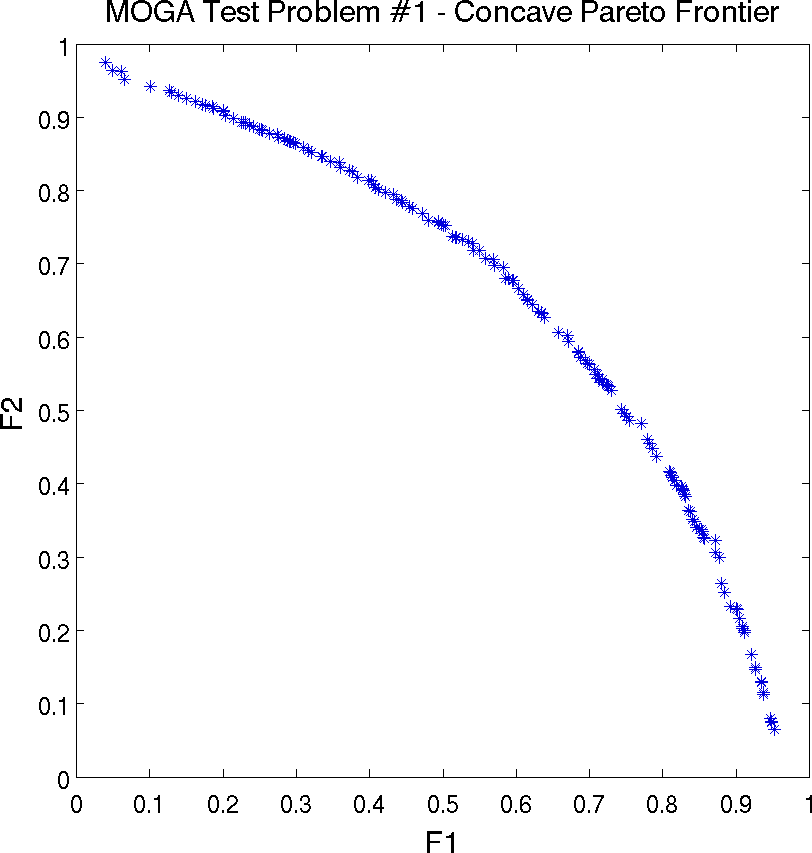
\includegraphics[scale=0.75]{images/dakota_mogatest1_pareto_front}
  \caption{Multiple objective genetic algorithm (MOGA) example: Pareto
  front showing tradeoffs between functions f1 and f2.}
  \label{additional:moga_pareto}
\end{figure}


%\subsection{Simultaneous Analysis and Design (SAND) Optimization}\label{opt:additional:sand}

%Dakota was originally developed as a ``black box'' optimization tool
%that employs non-intrusive interfaces with simulation codes. While
%this approach is useful for many engineering design applications, it
%can become prohibitively expensive when there is a large design space
%(i.e., $O(10^{2}-10^{6})$ design parameters) and when the
%computational simulation is highly nonlinear. Current research and
%development activities are investigating simultaneous analysis and
%design (SAND) methods, and these algorithms may be supported in Dakota
%in future releases. These ``all at once'' approaches are considerably
%more intrusive to a simulation code than any current interfacing
%capability in Dakota. But in some large-scale applications, the SAND
%method may be the only viable alternative for optimization.

%The basic idea behind SAND is to converge a nonlinear simulation code
%at the same time that the optimality conditions are being converged.
%This amounts to applying the nonlinear simulation residual equations
%as equality constraints in the optimization problem and then using an
%infeasible optimization method (e.g., sequential quadratic
%programming) which only satisfies these equality constraints in the
%limit (i.e., at the final optimal solution). This can result in a
%significant computational savings over black-box optimization
%approaches which require a nonlinear simulation to be fully-converged
%on every function evaluation.

%To implement a SAND technique, modifications to the simulation package
%are necessary so that the optimization software may have access to the
%internal residual vector and state Jacobian matrix used by the
%simulation solver. The SAND techniques can then leverage the internal
%linear algebra of the simulation package as appropriate in performing
%the search direction calculations. A SAND-type optimization does make
%certain assumptions about the simulation package, such as there is
%access to the state Jacobian matrix (although matrix free methods can
%be interfaced as well), exact values are used in the state Jacobian,
%an implicit numerical solution scheme is used, there are no
%discontinuities in the system, and steady state solutions are to be
%obtained (although SAND transient solution capabilities are under
%development). Many single physics, PDE-based simulation codes fall in
%this category. SAND approaches can be applied to more complex
%simulation codes, such as multi-physics packages, but substantial
%modifications are often needed to make SAND feasible in these cases.

%Details on SAND-type optimization approaches may be found
%in~\cite{Bar01a,Bir00}. Additional details on the SAND implementation
%in Dakota will appear in future releases of this Users Manual.

\subsection{Optimization with User-specified or Automatic Scaling}\label{opt:additional:scaling}

Some optimization problems involving design variables, objective
functions, or constraints on vastly different scales may be solved
more efficiently if these quantities are adjusted to a common scale
(typically on the order of unity). With any optimizer (or least
squares solver described in Section~\ref{nls:solution}),
user-specified characteristic value scaling may be applied to any of
continuous design variables, functions/residuals, nonlinear inequality
and equality constraints, and linear inequality and equality
constraints. Automatic scaling is available for variables or
responses with one- or two-sided bounds or equalities and may be
combined with user-specified scaling values. Logarithmic
($\log_{10}$) scaling is available and may also be combined with
characteristic values. Log scaling is not available for linear
constraints. Moreover, when continuous design variables are log
scaled, linear constraints are not permitted in the problem
formulation. Discrete variable scaling is not supported.

Scaling is enabled on a per-method basis for optimizers and least
squares minimizers by including the {\tt scaling} keyword in the
relevant {\tt method} specification in the Dakota input deck. When
scaling is enabled, variables, functions, gradients, Hessians, etc.,
are transformed such that the optimizer iterates in scaled variable
space, whereas evaluations of the computational model as specified in
the interface are performed on the original problem scale. Therefore
using scaling does not require rewriting the interface to the
simulation code. When the {\tt scaling} keyword is omitted, all {\tt
*\_scale\_types} and {\tt *\_scales} specifications described below
are ignored in the corresponding method, variables, and responses
sections. When the method {\tt output\_level} is set above normal,
scaling initialization and diagnostic information will be printed.

Scaling for a particular variable or response type is enabled through
the {\tt *\_scale\_types} specification (see the Reference Manual
method section and references contained therein for a complete keyword
list). Valid options for this string specification include {\tt
'none'} (default), {\tt 'value'}, {\tt 'auto'}, or {\tt 'log'}, for
no, characteristic value, automatic, or logarithmic scaling,
respectively (although not all types are valid for scaling all
entities). If a single string is specified with any of these keywords
it will apply to each component of the relevant vector, e.g., {\tt
cdv\_scale\_types = 'value'} will enable characteristic value scaling
for each continuous design variable.

The user may additionally specify no, one, or a vector of
characteristic scale values through the {\tt *\_scales} specification.
These characteristic values are ignored for scaling type {\tt 'none'},
required for {\tt 'value'}, and optional for {\tt 'auto'} and {\tt
'log'}. If a single value is specified with any of these keywords it
will apply to each component of the relevant vector, e.g., {\tt
cdv\_scales = 3.0} will apply a characteristic scaling value of 3.0 to
each continuous design variable.

When scaling is enabled, the following procedures determine the
transformations used to scale each component of a variables or
response vector. A warning is issued if scaling would result in
division by a value smaller in magnitude than {\tt 1.0e10*DBL\_MIN}.
User-provided values violating this lower bound are accepted
unaltered, whereas for automatically calculated scaling, the lower
bound is enforced.


\begin{itemize}

\item None ({\tt 'none'}): no scaling performed ({\tt *\_scales}
ignored) on this component.

\item Characteristic value ({\tt 'value'}): the corresponding quantity
      is scaled (divided) by the required characteristic value
      provided in the {\tt *\_scales} specification, and bounds are
      adjusted as necessary. If the value is negative, the sense of
      inequalities are changed accordingly.

\item Automatic ({\tt 'auto'}): First, any characteristic values from
      the optional {\tt *\_scales} specification are applied. Then,
      automatic scaling will be attempted according to the following
      scheme:

  \begin{itemize}
  
  \item two-sided bounds scaled into the interval [0,1];
	
  \item one-sided bounds or targets are scaled by a characteristic
    value to move the bound or target to 1, and the sense of
    inequalities are changed if necessary;

  \item no bounds or targets: no automatic scaling possible for this component
    
  \end{itemize}

  Automatic scaling is not available for objective functions nor least
  squares terms since they lack bound constraints. Further, when
  automatically scaled, linear constraints are scaled by
  characteristic values only, not affinely scaled into [0,1].

\item Logarithmic ({\tt 'log'}): First, any characteristic values from
the optional {\tt *\_scales} specification are applied. Then,
$\log_{10}$ scaling is applied. Logarithmic scaling is not available
for linear constraints. Further, when continuous design variables are
log scaled, linear constraints are not allowed.

\end{itemize}

Scaling for linear constraints specified through {\tt
linear\_inequality\_scales} or {\tt linear\_equality\_scales} is
applied {\em after} any (user-specified or automatic) continuous
variable scaling. For example, for scaling mapping unscaled
continuous design variables $x$ to scaled variables $\tilde{x}$:
\[ \tilde{x}^j = \frac{x^j - x^j_O}{x^j_M}, \]
where $x^j_M$ is the final component multiplier and $x^j_O$ the
offset, we have the following matrix system for linear inequality
constraints
\begin{eqnarray*}
& a_L \leq A_i x \leq a_U \\
& a_L \leq A_i \left( \mathrm{diag}(x_M) \tilde{x} + x_O \right) \leq a_U \\
& a_L - A_i x_O \leq A_i \mathrm{diag}(x_M) \tilde{x} \leq a_U - A_i x_O \\
& \tilde{a}_L \leq \tilde{A}_i \tilde{x} \leq \tilde{a}_U,
\end{eqnarray*}
and user-specified or automatically computed scaling multipliers are
applied to this final transformed system, which accounts for any
continuous design variable scaling. When automatic scaling is in use
for linear constraints they are linearly scaled by characteristic
values only, not affinely scaled into the interval $[0,1]$.

Figure~\ref{opt:additional:scaling:figure01} demonstrates the use of
several scaling keywords for the textbook optimization problem.
The continuous design variable {\tt x1} is scaled by a characteristic
value of 4.0, whereas {\tt x2} is scaled automatically into $[0,1]$
based on its bounds. The objective function will be scaled by a
factor of 50.0, then logarithmically, the first nonlinear constraint
by a factor of 15.0, and the second nonlinear constraint is not
scaled.

\begin{figure}
\centering
\begin{bigbox}
\begin{small}
\verbatimtabinput[8]{rosen_opt_scaled.in}
\end{small}
\end{bigbox}
\caption{Sample usage of scaling keywords in Dakota input specification.}
\label{opt:additional:scaling:figure01}
\end{figure}


\section{Optimization Usage Guidelines}\label{opt:usage}

In selecting an optimization method, important considerations include
the type of variables in the problem (continuous, discrete, mixed),
whether a global search is needed or a local search is sufficient, and
the required constraint support (unconstrained, bound constrained,
or generally constrained). Less obvious, but equally important,
considerations include the efficiency of convergence to an optimum
(i.e., convergence rate) and the robustness of the method in the
presence of challenging design space features (e.g., nonsmoothness).

Table~\ref{usage:guideopt} provides a convenient reference for
choosing an optimization method or strategy to match the
characteristics of the user's problem, where blank fields inherit the
value from above. With respect to constraint support, it should be
understood that the methods with more advanced constraint support are
also applicable to the lower constraint support levels; they are
listed only at their highest level of constraint support for brevity.

\begin{table}[hbp]
\centering
\caption{Guidelines for optimization method selection.}
\label{usage:guideopt}\vspace{2mm}
\begin{tabular}{|c|c|c|c|c|}
\hline
\textbf{Variable} & \textbf{Function} & \textbf{Solution} &
\textbf{Constraints} & \textbf{Applicable Methods} \\
\textbf{Type} & \textbf{Surface} & \textbf{Type} & & \\

\hline
continuous & smooth & local opt & none & optpp\_cg \\
\hline
      & & & bounds   & dot\_bfgs, dot\_frcg, conmin\_frcg \\
\hline
      & & & general  & npsol\_sqp, nlpql\_sqp, dot\_mmfd, dot\_slp, \\
      & & &          & dot\_sqp, conmin\_mfd, optpp\_newton, \\
      & & &          & optpp\_q\_newton, optpp\_fd\_newton \\
\hline
      & & local least sq & bounds  & nl2sol \\
\hline
      & &                & general & nlssol\_sqp, optpp\_g\_newton \\
\hline
      & & local multiobjective & general & weighted sums (one soln), \\
      & &                      &      & pareto\_set strategy (multiple solns) \\
%\hline
%     & & local large- & general & (planned: reduced\_sqp) \\
%     & & scale opt    &         &                         \\
\hline
      & & global opt      & general & hybrid strategy, multi\_start strategy \\
\hline
      & & global least sq & general & hybrid strategy, multi\_start strategy \\
%\hline
%      & nonsmooth & local opt & none & \\
\hline
      & nonsmooth & local opt & bounds & optpp\_pds \\
\hline
      & & & general & asynch\_pattern\_search, coliny\_cobyla, \\
      & & &         & coliny\_pattern\_search, coliny\_solis\_wets \\
\hline
      & & local/global opt      & general & surrogate\_based\_local \\
\hline
      & & local/global least sq & general & surrogate\_based\_local \\
\hline
      & & global opt            & bounds  & ncsu\_direct \\
\hline
      & &          & general & coliny\_ea, coliny\_direct, efficient\_global, \\
      & &          &         & soga, surrogate\_based\_global \\
\hline
  & & global least sq & general & efficient\_global, surrogate\_based\_global \\
\hline
      & & global multiobjective & general & moga (multiple solns) \\
\hline
discrete       & n/a & global opt & general  & soga, coliny\_ea \\
categorical    &     &            &          & \\
\hline
               &     & global multiobjective & general & moga (multiple solns)\\
\hline
discrete       & n/a & local opt  & general  & branch\_and\_bound strategy \\
noncategorical &     &            &          & \\
\hline
mixed          & nonsmooth & global opt & general & soga, coliny\_ea\\
categorical    &           &            &         & \\
\hline
               & & global multiobjective & general & moga (multiple solns) \\
\hline
mixed          & smooth  & local opt & general & branch\_and\_bound strategy \\
noncategorical &         &           &         & \\
\hline
\end{tabular}
\end{table}

{\bf Gradient-based Methods} \\
Gradient-based optimization methods are highly efficient, with the
best convergence rates of all of the optimization methods. If analytic
gradient and Hessian information can be provided by an application
code, a full Newton method will provide quadratic convergence rates
near the solution. More commonly, only gradient information is
available and a quasi-Newton method is chosen in which the Hessian
information is approximated from an accumulation of gradient data. In
this case, superlinear convergence rates can be obtained. These
characteristics make gradient-based optimization methods the methods
of choice when the problem is smooth, unimodal, and
well-behaved. However, when the problem exhibits nonsmooth,
discontinuous, or multimodal behavior, these methods can also be the
least robust since inaccurate gradients will lead to bad search
directions, failed line searches, and early termination, and the
presence of multiple minima will be missed.

Thus, for gradient-based optimization, a critical factor is the
gradient accuracy. Analytic gradients are ideal, but are often
unavailable. For many engineering applications, a finite difference
method will be used by the optimization algorithm to estimate gradient
values. Dakota allows the user to select the step size for these
calculations, as well as choose between forward-difference and
central-difference algorithms. The finite difference step size should
be selected as small as possible, to allow for local accuracy and
convergence, but not so small that the steps are ``in the noise.'' 
This requires an assessment of the local smoothness of the response
functions using, for example, a parameter study method. Central
differencing, in general, will produce more reliable gradients than
forward differencing, but at roughly twice the expense.

{\bf Non-gradient-based Methods} \\
Nongradient-based methods exhibit much slower convergence rates for
finding an optimum, and as a result, tend to be much more
computationally demanding than gradient-based methods. Nongradient
local optimization methods, such as pattern search algorithms, often
require from several hundred to a thousand or more function
evaluations, depending on the number of variables, and nongradient
global optimization methods such as genetic algorithms may require
from thousands to tens-of-thousands of function evaluations. Clearly,
for nongradient optimization studies, the computational cost of the
function evaluation must be relatively small in order to obtain an
optimal solution in a reasonable amount of time. In addition,
nonlinear constraint support in nongradient methods is an open area of
research and, while supported by many nongradient methods in Dakota,
is not as refined as constraint support in gradient-based
methods. However, nongradient methods can be more robust and more
inherently parallel than gradient-based approaches. They can be
applied in situations were gradient calculations are too expensive or
unreliable. In addition, some nongradient-based methods can be used
for global optimization which gradient-based techniques, by
themselves, cannot. For these reasons, nongradient-based methods
deserve consideration when the problem may be nonsmooth, multimodal,
or poorly behaved.

{\bf Surrogate-based Methods} \\
Approaches that seek to improve the effectiveness or efficiency of
optimizers and least squares methods through the use of surrogate
models include the surrogate-based local, surrogate-based global, and
efficient global methods. Chapter~\ref{sbm} provides further
information on these approaches. The surrogate-based local approach
(see Section~\ref{sbm:sblm}) brings the efficiency of gradient-based
optimization/least squares methods to nonsmooth or poorly behaved
problems by smoothing noisy or discontinuous response results with a
data fit surrogate model (e.g., a quadratic polynomial) and then
minimizing on the smooth surrogate using efficient gradient-based
techniques. The surrogate-based global approach (see
Section~\ref{sbm:sbgm}) similarly employs optimizers/least squares
methods with surrogate models, but rather than localizing through the
use of trust regions, seeks global solutions using global methods.
And the efficient global approach (see Section~\ref{sbm:egm}) uses the
specific combination of Gaussian process surrogate models in
combination with the DIRECT global optimizer. Similar to these
surrogate-based approaches, the hybrid and multistart optimization
strategies seek to bring the efficiency of gradient-based optimization
methods to global optimization problems. In the former case, a global
optimization method can be used for a few cycles to locate promising
regions and then local gradient-based optimization is used to
efficiently converge on one or more optima. In the latter case, a
stratification technique is used to disperse a series of local
gradient-based optimization runs through parameter space. Without
surrogate data smoothing, however, these strategies are best for
smooth multimodal problems. Section~\ref{strat:hybrid} and
Section~\ref{strat:multistart} provide more information on these
approaches.

\section{Additional Examples}\label{opt:examples}

\subsection{Nongradient-based Optimization via Pattern Search}\label{opt:examples:ps}

In addition to gradient-based optimization algorithms, Dakota also
contains a variety of nongradient-based algorithms. One particular
nongradient-based algorithm for local optimization is known as pattern
search (see Chapter~\ref{intro} for a discussion of local
versus global optimization). The Dakota input file shown in
Figure~\ref{opt:examples:psfig} applies a pattern
search method to minimize the Rosenbrock function. While this
provides for an interesting comparison to the previous example
problems in this chapter, the Rosenbrock function is not the best test
case for a pattern search method. That is, pattern search methods are
better suited to problems where the gradients are too expensive to
evaluate, inaccurate, or nonexistent --- situations common among many
engineering optimization problems. It also should be noted that
nongradient-based algorithms generally are applicable only to
unconstrained or bound-constrained optimization problems, although the
inclusion of general linear and nonlinear constraints in
nongradient-based algorithms is an active area of research in the
optimization community. For most users who wish to use
nongradient-based algorithms on constrained optimization problems, the
easiest route is to create a penalty function, i.e., a composite
function that contains the objective function and the constraints,
external to Dakota and then optimize on this penalty function. Most
optimization textbooks will provide guidance on selecting and using
penalty functions.

The Dakota input file shown in Figure~\ref{opt:examples:ps} is similar
to the input file for the gradient-based optimization, except it has a
different set of keywords in the method block of the input file, and
the gradient specification in the responses block has been changed to
\texttt{no\_gradients}. The pattern search optimization algorithm used
is part of the SCOLIB library~\cite{Har06}. See the Dakota Reference
Manual~\cite{RefMan} for more information on the \emph{methods} block
commands that can be used with SCOLIB algorithms.

\begin{figure}[ht!]
  \centering
  \begin{bigbox}
    \begin{small}
      \verbatimtabinput[8]{rosen_opt_patternsearch.in}
    \end{small}
  \end{bigbox}
  \caption{Rosenbrock pattern search optimization example: the Dakota input file.}
  \label{opt:examples:psfig}
\end{figure}

For this run, the
optimizer was given an initial design point of $(x_1,x_2)
  = (0.0,0.0)$ and was limited to 2000 function evaluations. In this
case, the pattern search algorithm stopped short of the optimum at
$(x_1,x_2) = (1.0,1,0)$, although it was making progress
in that direction when it was terminated. (It would have
reached the minimum point eventually.)

The iteration history is provided in Figures~
\ref{opt:examples:ps_graphics}(a) and (b), which show
the locations of the function evaluations used in the pattern search
algorithm.
Figure~\ref{opt:examples:ps_graphics}(c)
provides a close-up view of the pattern search function evaluations
used at the start of the algorithm. The coordinate pattern is clearly
visible at the start of the iteration history, and the decreasing size
of the coordinate pattern is evident at the design points move toward
$(x_1,x_2) = (1.0,1.0)$.

\begin{figure}[ht!]
  \centering
  \begin{tabular}{cc}
  \multicolumn{2}{c}
	      {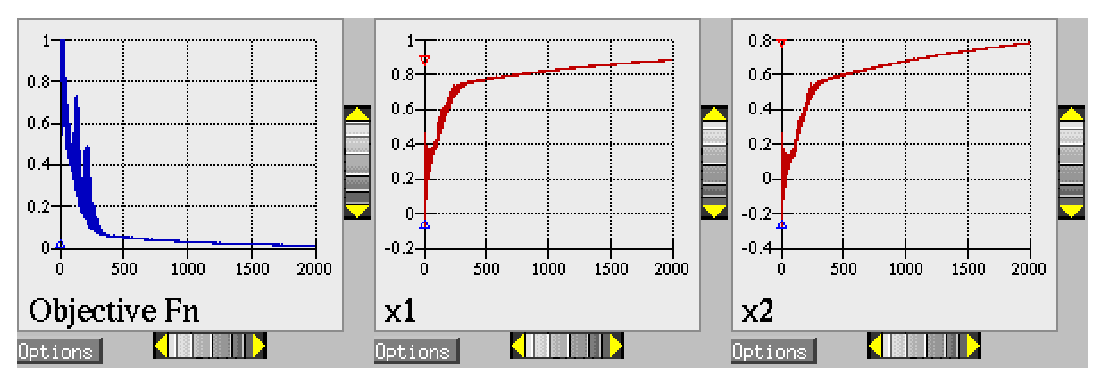
\includegraphics[width=\textwidth]{images/dak_graphics_ps_opt}}\\
  \multicolumn{2}{c}{(a)}\\
  \qquad\\
  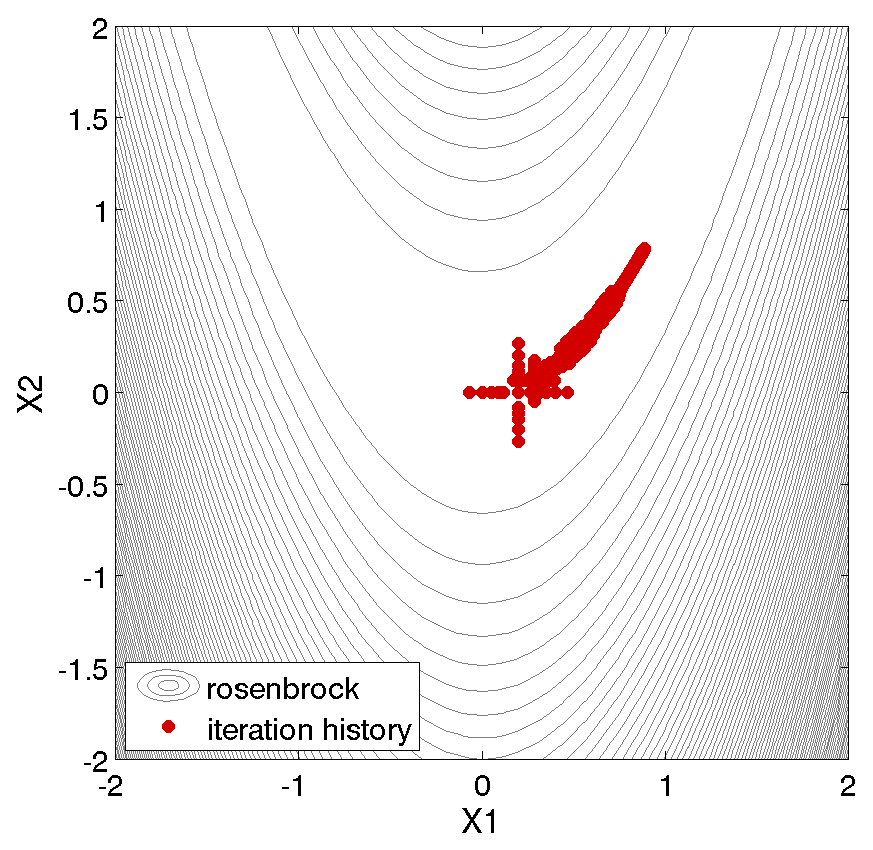
\includegraphics[height=2.5in]{images/rosen_ps_opt_pts} &
  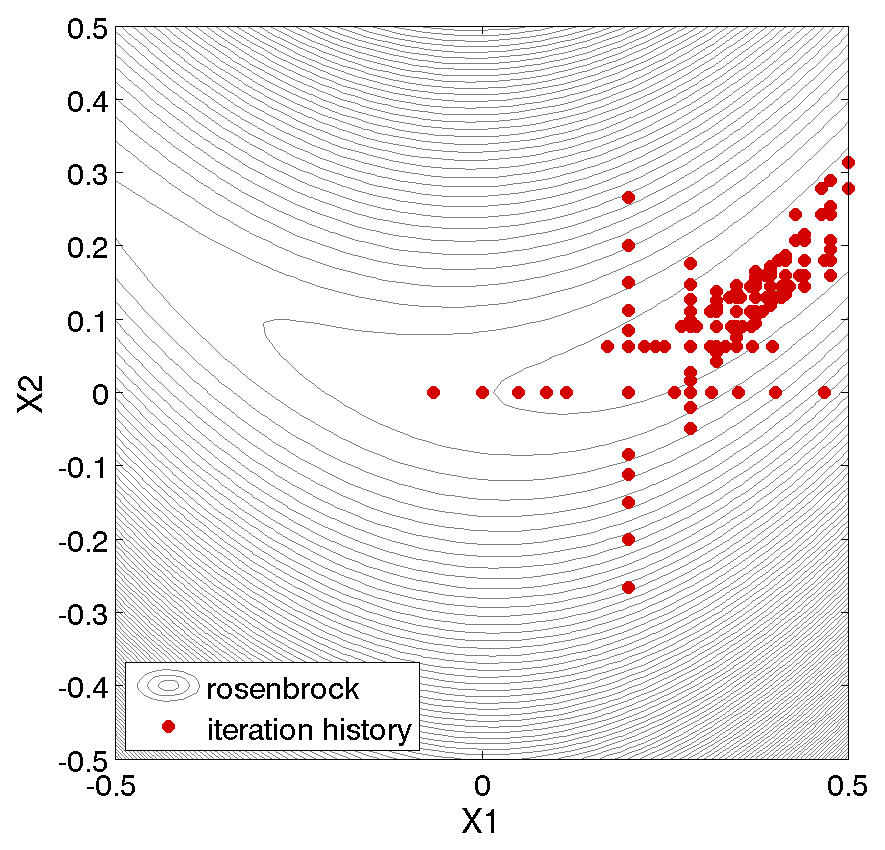
\includegraphics[height=2.5in]{images/rosen_ps_opt_pts2} \\
  (b) & (c)
  \end{tabular}
  \caption{Rosenbrock pattern search optimization example: (a) screen
    capture of the Dakota graphics, (b) sequence of design points
    (dots) evaluated and (c) close-up view illustrating the shape of
    the coordinate pattern used. }
  \label{opt:examples:ps_graphics}
\end{figure}

While pattern search algorithms are useful in many optimization
problems, this example shows some of the drawbacks to this algorithm.
While a pattern search method may make good initial progress towards
an optimum, it is often slow to converge. On a smooth, differentiable
function such as Rosenbrock's function, a nongradient-based method
will not be as efficient as a gradient-based method. However, there
are many engineering design applications where gradient information is
inaccurate or unavailable, which renders gradient-based optimizers
ineffective. Thus, pattern search algorithms (and other
nongradient-based algorithms such as genetic algorithms as discussed in the
next section) are often good choices in complex engineering applications
when the quality of gradient data is suspect.

\subsection{Nongradient-based Optimization via Evolutionary Algorithm}\label{opt:examples:ea}

In contrast to pattern search algorithms, which are local optimization
methods, evolutionary algorithms (EA) are global optimization
methods. As was described above for the pattern search algorithm, the
Rosenbrock function is not an ideal test problem for showcasing the
capabilities of evolutionary algorithms. Rather, EAs are best suited
to optimization problems that have multiple local optima, and where
gradients are either too expensive to compute or are not readily available.

Evolutionary algorithms are based on Darwin's theory of survival of
the fittest. The EA algorithm starts with a randomly selected
population of design points in the parameter space, where the values
of the design parameters form a ``genetic string,'' analogous
to DNA in a biological system, that uniquely represents each design
point in the population. The EA then follows a sequence of
generations, where the best design points in the population (i.e.,
those having low objective function values) are considered to be the
most ``fit'' and are allowed to survive and reproduce. The EA
simulates the evolutionary process by employing the mathematical
analogs of processes such as natural selection, breeding, and
mutation. Ultimately, the EA identifies a design point (or a family of
design points) that minimizes the objective function of the
optimization problem. An extensive discussion of EAs is beyond the
scope of this text, but may be found in a variety of sources (cf.,
~\cite{Haf92} pp. 149-158;~\cite{Gol89}). Currently, the EAs available
in Dakota include a genetic algorithm for problems involving discrete
variables and an evolution strategy with self-adaptation for problems
with continuous variables. Details of these algorithms are given in
the Dakota Reference Manual~\cite{RefMan}. The SCOLIB library, which
provides the EA software that has been linked into Dakota, is
described in~\cite{Har06}.

\begin{figure}[ht!]
  \centering
  \begin{bigbox}
    \begin{small}
      \verbatimtabinput[8]{rosen_opt_ea.in}
    \end{small}
  \end{bigbox}
  \caption{Rosenbrock evolutionary algorithm optimization example: the
  Dakota input file.}
  \label{opt:examples:rosenbrock_ea}
\end{figure}

Figure~\ref{opt:examples:rosenbrock_ea} shows a Dakota input file that
uses an EA to minimize the Rosenbrock function. For this
example the EA has a population size of 50. At the start of the first
generation, a random number generator is used to select 50 design
points that will comprise the initial population. \emph{[A specific
  seed value is used in this example to generate repeatable results,
  although, in general, one should use the default setting which
  allows the EA to choose a random seed.]} A two-point crossover
technique is used to exchange genetic string values between the
members of the population during the EA breeding process. The result
of the breeding process is a population comprised of the 10 best
``parent'' design points (elitist strategy) plus 40 new ``child''
design points. The EA optimization process will be terminated after
either 100 iterations (generations of the EA) or 2,000 function
evaluations. The EA software available in Dakota provides the user
with much flexibility in choosing the settings used in the
optimization process. See~\cite{RefMan} and~\cite{Har06} for details on these
settings.

The EA optimization results
printed at the end of this file show that the best design point found
was $(x_1,x_2) = (0.98,0.95)$. The file
\texttt{ea\_tabular.dat.sav} provides a listing of the design
parameter values and objective function values for all 2,000 design
points evaluated during the running of the EA. Figure~
\ref{opt:examples:rosenbrock_ea_graphics}(a) shows the population of
50 randomly selected design points that comprise the first generation
of the EA, and Figure~\ref{opt:examples:rosenbrock_ea_graphics}(b)
shows the final population of 50 design points, where most of the 50
points are clustered near $(x_1,x_2) = (0.98,0.95)$.

\begin{figure}[hbt!]
  \centering
  \begin{tabular}{cc}
  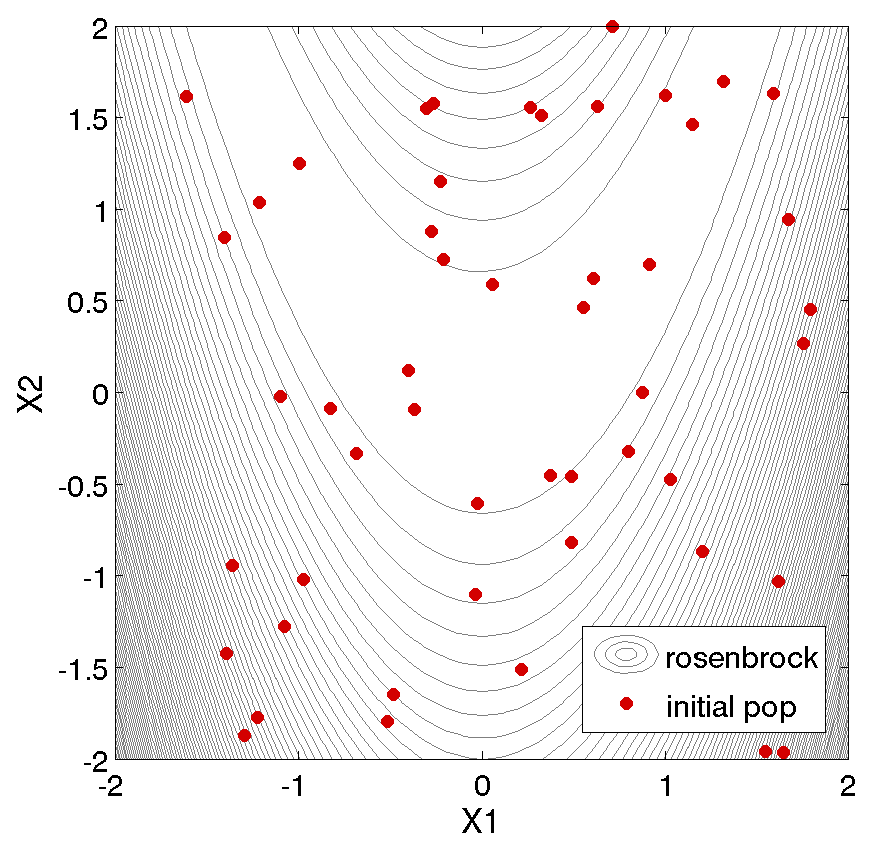
\includegraphics[height=2.5in]{images/rosen_ea_init} &
  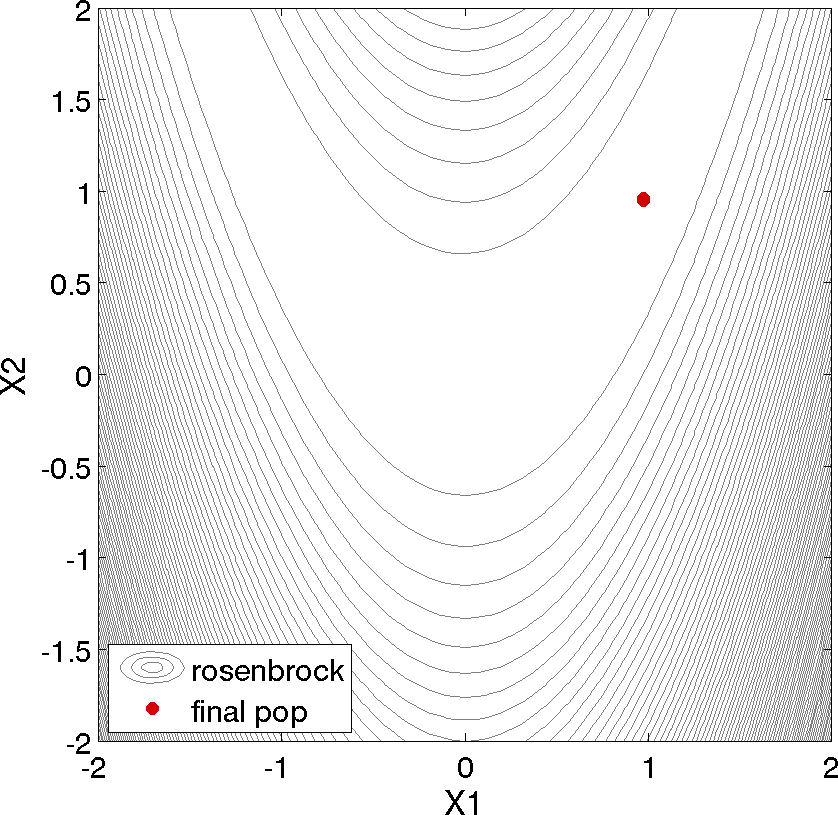
\includegraphics[height=2.5in]{images/rosen_ea_final} \\
  (a) & (b)
  \end{tabular}
  \caption{Rosenbrock evolutionary algorithm optimization example: 50
    design points in the (a) initial and (b) final populations
    selected by the evolutionary algorithm. }
  \label{opt:examples:rosenbrock_ea_graphics}
\end{figure}

As described above, an EA is not well-suited to an optimization
problem involving a smooth, differentiable objective such as the
Rosenbrock function. Rather, EAs are better suited to optimization
problems where conventional gradient-based optimization fails, such as
situations where there are multiple local optima and/or gradients are
not available. In such cases, the computational expense of an EA is
warranted since other optimization methods are not applicable or
impractical. In many optimization problems, EAs often quickly identify
promising regions of the design space where the global minimum may be
located. However, an EA can be slow to converge to the optimum. For
this reason, it can be an effective approach to combine the global
search capabilities of a EA with the efficient local search of a
gradient-based algorithm in a \emph{hybrid optimization} strategy. In
this approach, the optimization starts by using a few iterations of a
EA to provide the initial search for a good region of the parameter
space (low objective function and/or feasible constraints), and then
it switches to a gradient-based algorithm (using the best design point
found by the EA as its starting point) to perform an efficient local
search for an optimum design point. More information on this hybrid
approach is provided in Chapter~\ref{strat}.

In addition to the evolutionary algorithm capabilities in the
\texttt{coliny\_ea} method, there is a single-objective genetic algorithm
method called \texttt{soga}.
%The major differences are that
%\texttt{soga} allows a warm start (e.g., you can read in starting
%solutions from a file), and it allows one to specify a mix of
%continuous and discrete design variables.
For more information on \texttt{soga}, see Chapter~\ref{opt}.
